\documentclass[11pt]{amsart}
\usepackage{amsmath}
\usepackage{geometry}                % See geometry.pdf to learn the layout options. There are lots.
\geometry{letterpaper}                   % ... or a4paper or a5paper or ... 
%\geometry{landscape}                % Activate for for rotated page geometry
%\usepackage[parfill]{parskip}    % Activate to begin paragraphs with an empty line rather than an indent
\usepackage{graphicx}
\usepackage{caption}
\usepackage{subcaption}
\usepackage{amssymb}
\usepackage{epstopdf}
\usepackage[]{algorithm2e}

\graphicspath{{../Figures/}}

\DeclareGraphicsRule{.tif}{png}{.png}{`convert #1 `dirname #1`/`basename #1 .tif`.png}

\newcommand{\vek}[1]{\mathbf{#1}}
\newcommand{\norm}[1]{\left\lVert#1\right\rVert}

\title{COMP 652: Assignment 1}
\author{Carlos G. Oliver \\ 260425853}
\date{\today}                                           % Activate to display a given date or no date

\begin{document}
\maketitle
\section{Regression}
\subsection{Q1 (c):Objective for logistic regression with $L_{2}$ regulariztion.}

The logistic regression objective is the cross entropy error function between true outputs $y_i$ and predictions $h(x_i)$ with the additional regularization term proportional to some constant $\lambda$ and the $L_2$ norm of the weight vector $\vek{w}$.
\begin{equation}
J_{\vek{w}} =  -\bigg(\sum_{i=1}^{m} y_{i}\log(h(\vek{x_{i}})) + (1 - y_{i})\log(1 - h(\vek{x_{i}}))\bigg) + \frac{\lambda}{2}\vek{w}^T\vek{w}
\end{equation}

\subsection{Q1 (d): Regularization}

For all subsequent experiments, I present summary statistics of K-fold cross validation with shuffled input data. We compute a value of $K$ so as to have approximately a training-test split ratio of $80-20\%$. This resulted in $4$ splits. The bars one each point represent one standard deviation from the mean over the $4$ splits. 

\begin{figure}
    \centering
    \begin{subfigure}{0.45\textwidth}
        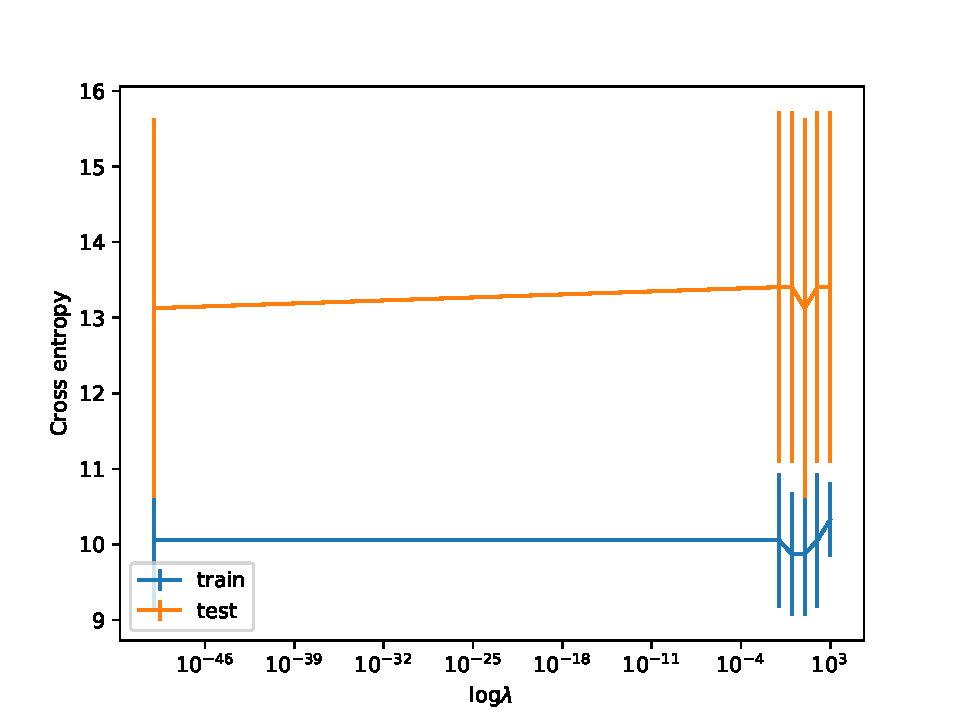
\includegraphics[width=\textwidth]{q1d_crossentropy.pdf}
        \caption{MFE Sampling}
        \label{fig:rnamutsnomfe_freq}
    \end{subfigure}
    \begin{subfigure}{0.45\textwidth}
        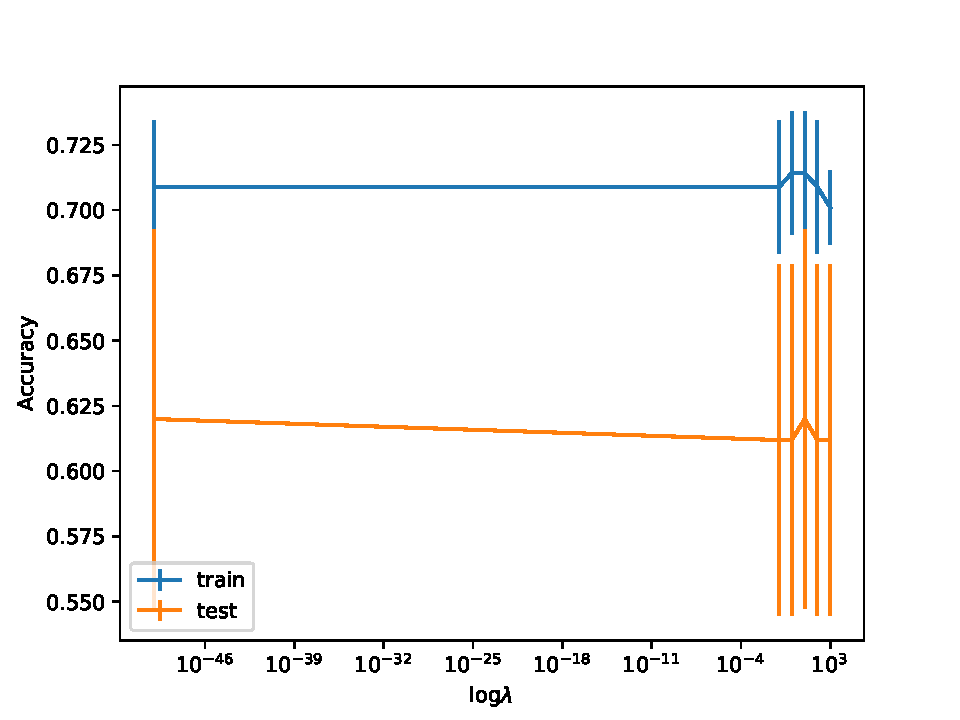
\includegraphics[width=\textwidth]{q1d_accuracy.pdf}
        \caption{Suboptimal Sampling}
        \label{fig:ranmutsnomfe_freq}
    \end{subfigure}
    \begin{subfigure}{0.45\textwidth}
        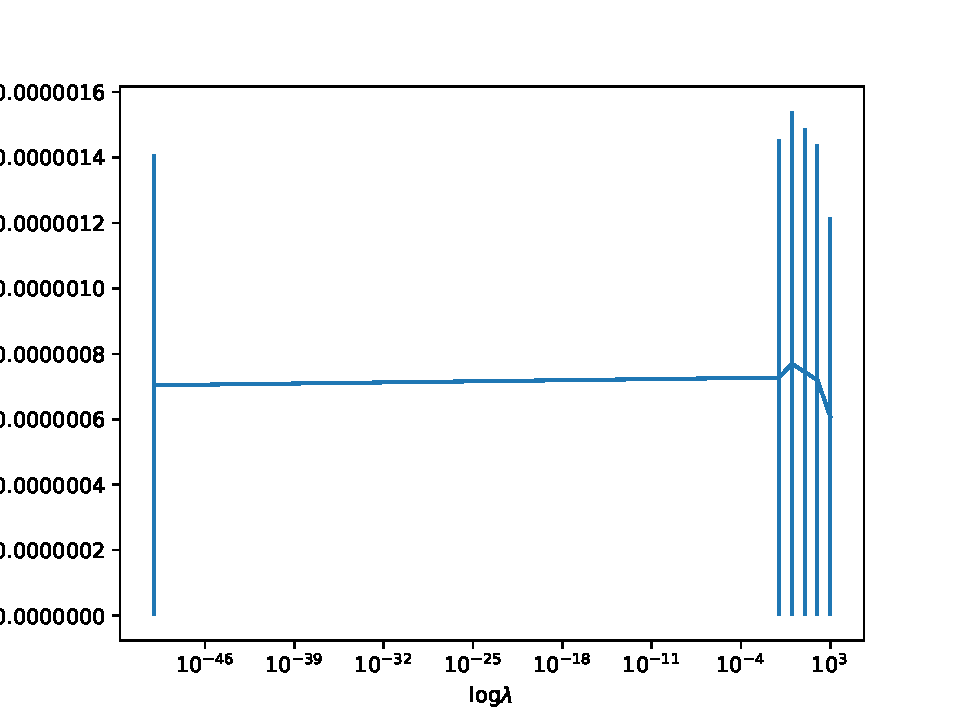
\includegraphics[width=\textwidth]{q1d_norm.pdf}
        \caption{Suboptimal Sampling}
        \label{fig:ranmutsnomfe_freq}
    \end{subfigure}
    \begin{subfigure}{0.45\textwidth}
        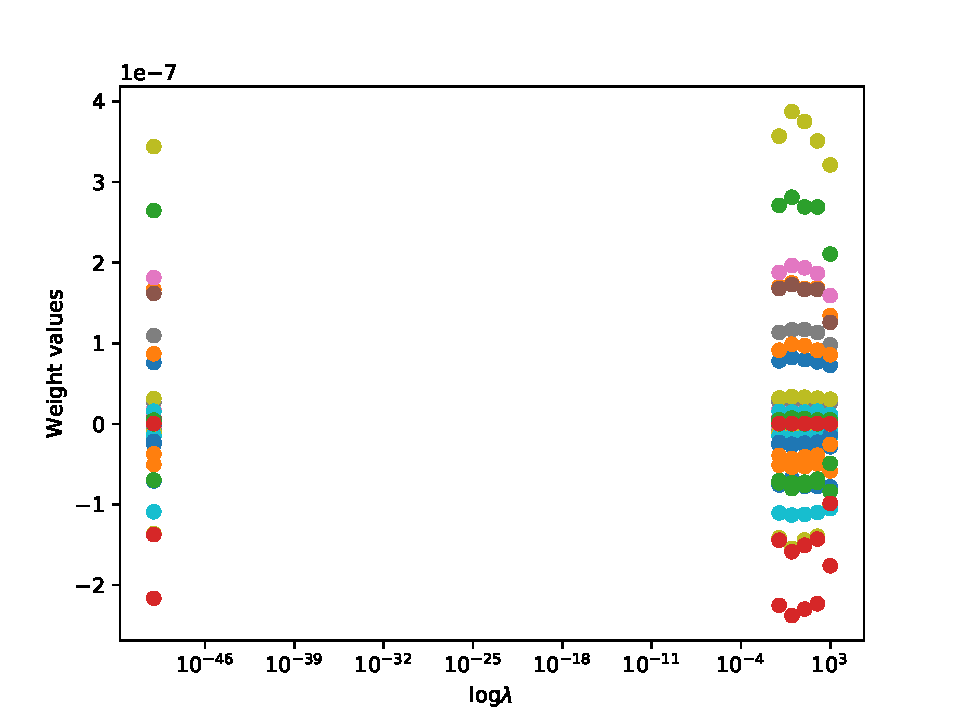
\includegraphics[width=\textwidth]{q1d_weights.pdf}
        \caption{Suboptimal Sampling}
        \label{fig:ranmutsnomfe_freq}
    \end{subfigure}
        \caption{Frequency of sequence-structure pair in Boltzmann ensemble for MFE and suboptimal sampling in RNAmutants.}
    \label{fig:freq}
\end{figure}


\subsection{Q1 (e): Gaussian Basis Functions}

Next, we apply a univariate Gaussian basis function $\phi_j(x_i)$ to each value in input vectors $x$ to compute a new feature mapping. Where

\begin{equation}
	\phi(x)_j = exp\bigg[{\frac{(x_i - \mu_k)^2}{2\sigma^2}}\bigg]
\end{equation}

We apply this basis with a fixed $\sigma$ chosen from the set $\{0.1, 0.5, 1, 5, 10\}$ at each iteration. For each variable we compute $5$ basis functions ($\phi_{1}(x), ... \phi_{5}(x)$) with $\mu \in \{-10, -5, 0, 5, 10\}$ resulting in 5 feature vectors for each original feature vector in $X$. This results in a new input matrix $\Phi$.

\subsection{Q1 (f): Effect of $\sigma$ on regression}

\begin{figure}
	\centering
	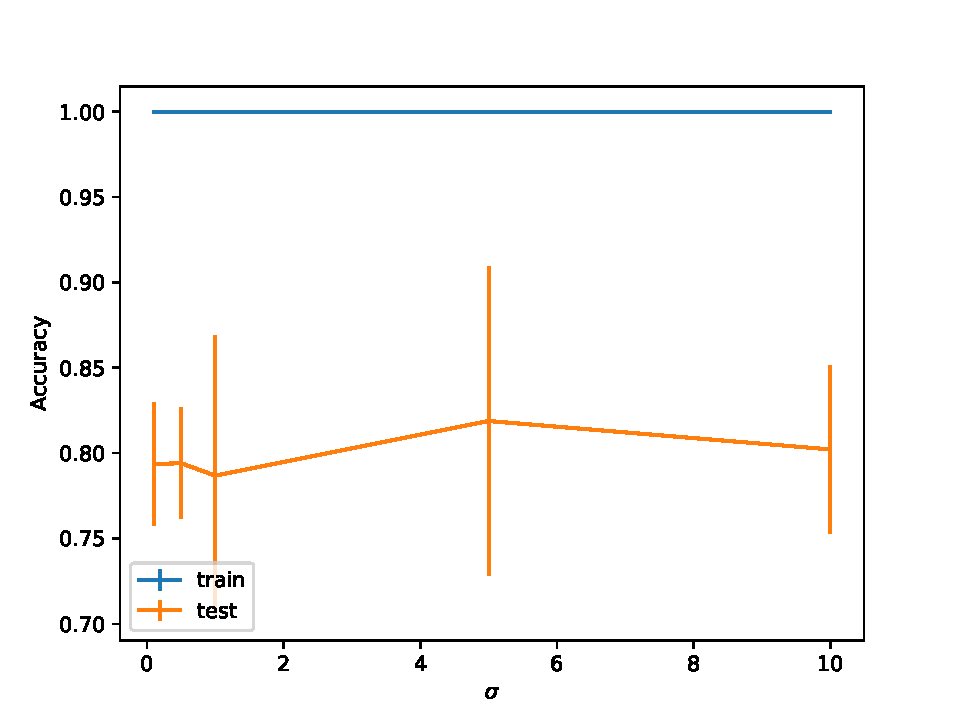
\includegraphics[width=0.45\textwidth]{sigmas.pdf}
\end{figure}

\subsection{Q1 (g): Basis function and regularization}

%\begin{figure}
%	\centering
%	\begin{subfigure}
%		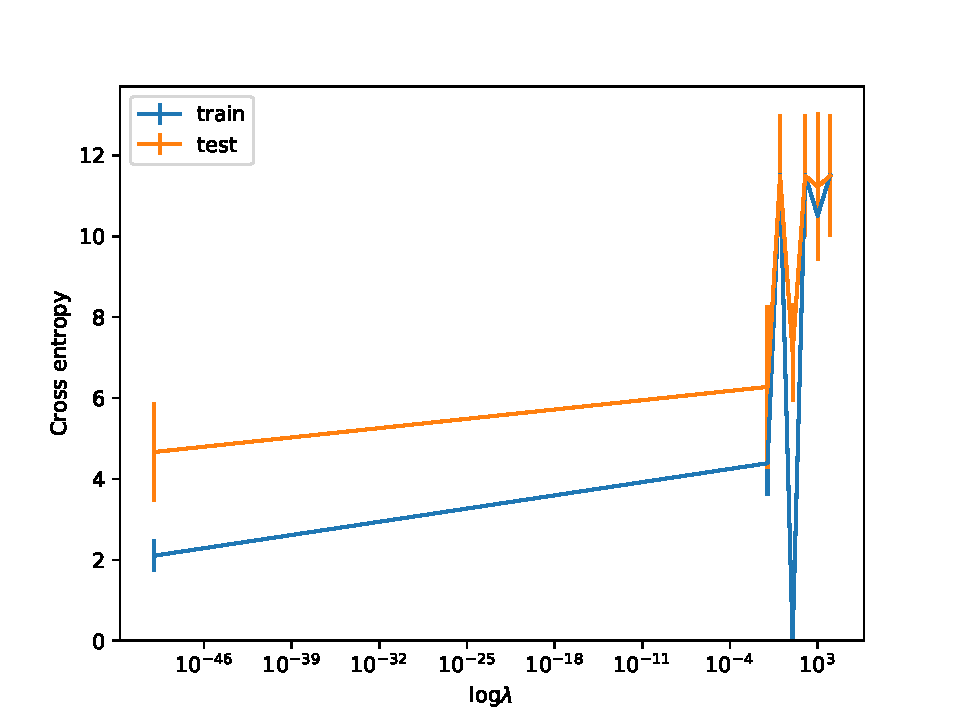
\includegraphics[width=0.45\textwidth]{all_sigmas.pdf}
%		\caption{Average cross entropy}
%	\end{subfigure}
%
%	\begin{subfigure}
%		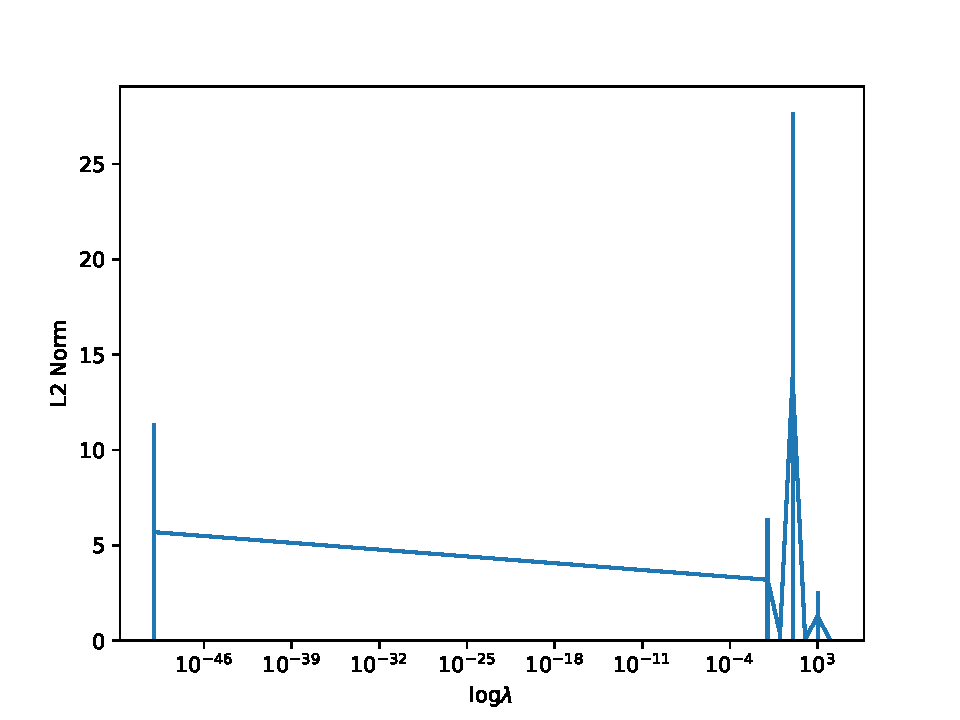
\includegraphics[width=0.45\textwidth]{all_sigmas_norm.pdf}
%		\caption{L2 norm of weight vector}
%	\end{subfigure}
%\end{figure}

\subsection{Q1 (h): Gaussian basis function capturing relationship between inputs}

Instead of using a univariate Gaussian basis function to transform each input variable, we could use multivariate Gaussians to capture the relationship between inputs as covariance. We can use a similar basis as before, but introduce a covariance parameter matrix $\Sigma$ that can be estimated from the data. As we would be increasing the complexity of our model, we are likely to reduce the bias but make the model more sensitive to variations in the data. 

\subsection{Q1 (i): Adaptive gaussian center placement}

Previously, we have been externally fixing the centers $\mu_i$ of the Gaussian basis functions. We can instead use the data to adaptively compute the placement of these centers. This would effectively be a clustering task, where each cluster would define the center of a Gaussian basis. With a fixed $\sigma$, the only parameter we need to estimate is the center vector $\mu$ for each center $k$. Our basis functions would then take the form:

\begin{equation}
\phi(\vek{x}) = exp\bigg(\frac{\norm{\vek{x} - \mathbf{\mu}}_2^2}{2\sigma_k^2}\bigg)
\end{equation}

\IncMargin{1em}
\begin{algorithm}[H]
	\SetKwInOut{Input}{input}\SetKwInOut{Output}{output}
	\SetKwFunction{KMeans}{KMeans}
	\SetKwFunction{GaussianBasis}{GaussianBasis}
	\SetKwFunction{LogisticRegression}{LogisticRegression}
	\SetKwFunction{accuracy}{accuracy}

	\Input{X, $\lambda$, $\vek{y}$, [$\sigma_0$, ..., $\sigma_j$]}
	\Output{$\vek{\omega}$}
	
	$currentTestErr \leftarrow \infty$\;
	$prevTestErr \leftarrow 0$\;
	$bestMode \leftarrow Null$\;
	\While{$currentTestErr > prevTestErr$}{
		$\mu_1, ..., \mu_j \leftarrow$ \KMeans{X, k}\; 
		$X^{'} \leftarrow$ \GaussianBasis{$X, [\mu_1, ..., \mu_k]$}\;
		$model, \vek{w} \leftarrow$ \LogisticRegression{$X^{'}, y, \lambda$}\;
		$currentTestErr \leftarrow \accuracy{model, X, y}$;
	}
	

\end{algorithm}
\subsection{Q1 (j): Convergence of algorithm}



\subsection{Q2 (a): Dual view of logistic regression}

The hypothesis $h(\vek{x})$ in logistic regression takes the form:

\begin{equation}
h(\vek{x}) = P(Y=1 \vert \vek{x}, \vek{w}) = \frac{1}{1 + e^{\vek{w^T}\vek{x}}}
\end{equation}

If we wish to obtain the probability distribution of $y$ condition on $\vek{x}$ and $\vek{w}$ we get:

\begin{equation}
p(y \vert \vek{x}, \vek{w}) = \sigma(y\vek{w^T}\vek{x}) = \frac{1}{1 + e^{-y\vek{w^T}\vek{x}}}
\end{equation}

We can then use this form to find the parameters that maximize the log likelihood of the data given a choice of model. (The following derivation is based on work published by Thomas P. Minka in 2007 \cite{minka2003comparison}.)

\begin{equation}
l(\vek{w}) = \sum_{i=1}^{m} \log\sigma(-y_i\vek{w^T}\vek{x}) - \frac{\lambda}{2}\vek{w^T}\vek{w}
\end{equation}

In order to derive a dual expression of this objective, we aim to find a tight linear upper bound parametrized by a new set of parameters $\alpha_{i}$. Such a function will let us reverse the order of the optimization while maintaining the same optima. In our case, if we wish to maximize $l(\vek{w})$ we can instead minimize some function $l(\vek{w}, \vek{\alpha})$ that is an upper bound to the first. We can then find the minimal value of $l(\vek{w}, \vek{\alpha})$ that maximizes $l(\vek{w})$.

We use the function:

\begin{equation}
H(\alpha) = -\alpha\log\alpha - (1-\alpha)\log(1-\alpha), \quad \alpha \in [0, 1]
\end{equation}

Plotting $H(x)$ we see that the function is quadratic.

\begin{figure}[h]
	\centering
	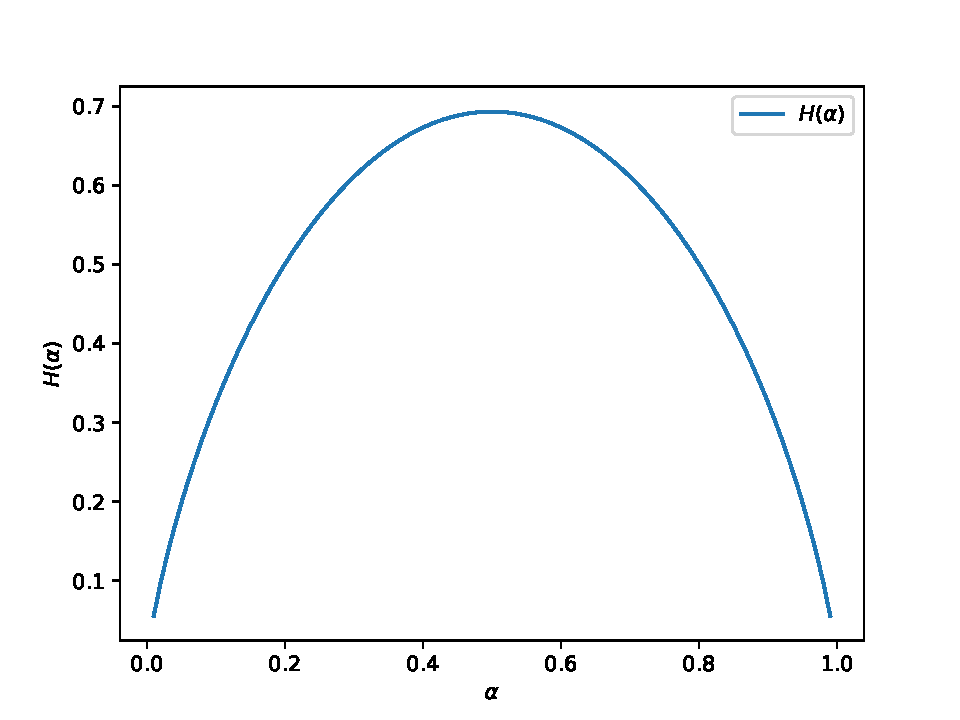
\includegraphics[width=0.45\textwidth]{H_x.pdf}
	\caption{Parameter function}
\end{figure}

Using $H(x)$ we can bound $\log(\sigma(x))$ above as follows:

\begin{equation}
\log\sigma(x) \leq \alpha x - H(x)
\end{equation} 

Plotting these functions with $\alpha = \{0, 0.5, 1\}$ we see that indeed, $\log\sigma(x)$ is tightly bounded above.

\begin{figure}
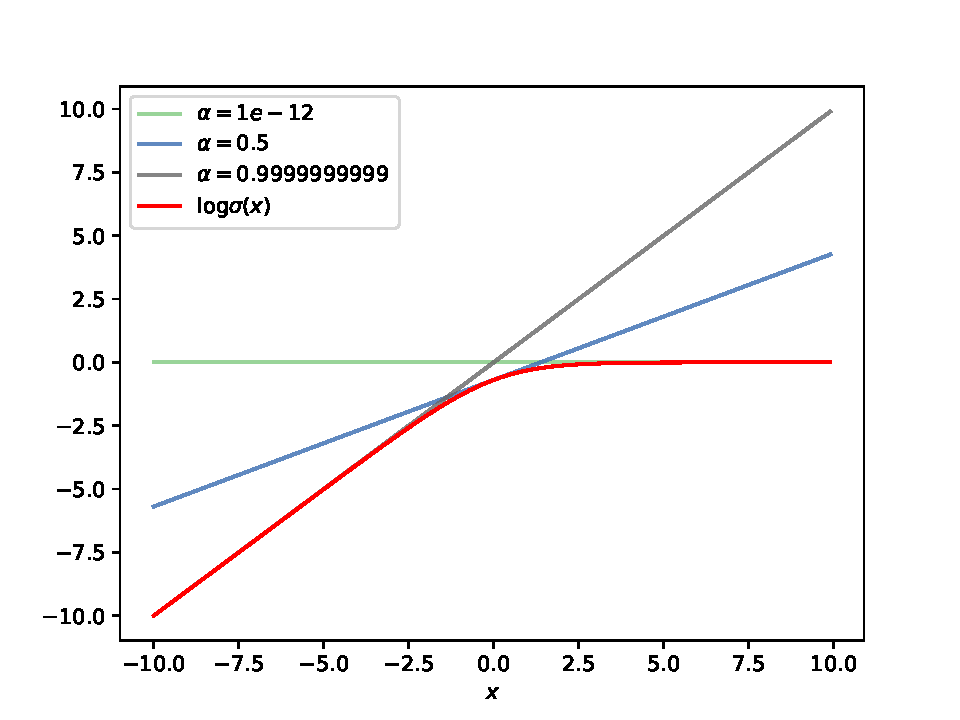
\includegraphics[width=0.45\textwidth]{bounds.pdf}
\caption{Upper bounds on log likelihood function}
\end{figure}

We can then apply these constraints to the original log likelihood function optimization problem:

\begin{equation}
l(\vek{w}) = \sum_{i}^{m} \log \sigma(y_i\vek{w^T}\vek{x}) - \frac{\lambda}{2}\vek{w^T}\vek{w} \leq l(\vek{w}, \vek{\alpha})
\end{equation}

\begin{equation}
\text{Where}\quad l(\vek{w}, \vek{\alpha}) = \sum_{i}^{m} \alpha_{i}y_{i}\vek{w^Tx_i} - H(\alpha_i) - \frac{\lambda}{2}\vek{w^Tw}
\end{equation}

We can now write the problem as a minimization problem over $\vek{\alpha}$

\begin{equation}
\min_{\alpha}\max_{\vek{w}} l(\vek{w}, \vek{\alpha})
\end{equation}

Taking the derivative of $l(\vek{w}, \alpha)$ with respect to $\vek{w}$ and setting to zero we get an expression for $\vek{w}$

\begin{equation}
\vek{w(\alpha)} = -\lambda\sum_{i}^{m}\alpha_{i}y_{i}\vek{x_i}
\end{equation}

Which we can plug into the original $l(\vek{w}, \vek{\alpha})$ and now optimize with respect to $\alpha$ to obtain

\begin{equation}
J(\vek{\alpha}) = \frac{1}{2\lambda}\sum_{i,j}^{m,n}\alpha_{i}\alpha_{j}y_{i}y_{j}\vek{x_{j}^{T}\cdot x_{i}} - \sum_{i}^{m}H(\alpha_i)
\end{equation}

This is the dual view of logistic regression, where the objective is expressed in terms of weighted dot products between input instances and not in terms of weight vector $\vek{w}$. In this form, we can apply any valid kernel to the dot product $\vek{x_i^T\cdot x_j}$ as $K(\vek{x_i, x_j)}$. It is important to note that $\vek{\alpha} \in \mathbb{R}^m$ where $m$ is the number of input instances, and $\vek{w} \in \mathbb{R}^n$ where $n$ is the number of features. When using kernel methods $n$ can grow exponentially, making the dual form more computationally tractable when the number of instances is low compared to the number of features. 

In order to solve for the optimal $\vek{\alpha}$ Minka proposes to use coordinate wise Newton method instead of Newton's method to avoid inverting the Hessian. 

\begin{equation}
g_i = \frac{dJ(\vek{\alpha})}{d\alpha_i} = y_i\vek{w(\alpha)}^T x_i + \log \bigg(\frac{\alpha}{1-\alpha_i}\bigg)
\end{equation}

Using the first derivative we can iteratively step in the direction of the gradient over each $\alpha_i$.

\begin{equation}
\alpha_i^{new} = \alpha_i - \frac{g_i}{\lambda^{-1}\vek{x_i}^T\vek{x_i} + \frac{1}{\alpha_i(1-\alpha_i)}}
\end{equation}

Having obtained the vector $\vek{\alpha}$ through this procedure, we can make predictions using the original logistic model with a kernel.

\begin{equation}
P(Y=1 \vert x, \alpha) = \sigma\bigg(\sum_i^{m} \alpha_i K(\vek{x}, \vek{x_i})\bigg)
\end{equation}


\subsection{Q2 (b): Implementation of kernelized logistic regression}


\subsection{Q2 (c): Kernelized logistic regression vs. non-kernel logistic regression results}


\subsection{Q2 (d): Advantages and disadvantages of kernelized logistic regression}

\subsection{Q3: (a) Kernels}

{\it Statement:} $K(\vek{x}, \vek{z}) = aK_1(\vek{x}, \vek{z}) + bK_{2}(\vek{x}, \vek{z})$ is a kernel given that $K_1$ and $K_2$ are kernels and $a,b \in \mathbb{R}$ and $a, b > 0$.

\begin{proof}

If $K_1$ and $K_2$ are kernels then we can write them as:

\begin{equation}
K_1(\vek{x}, \vek{z}) = \phi^1(\vek{x})^T\phi^1(\vek{z})
\end{equation}

\begin{equation}
K_2(\vek{x}, \vek{z}) = \phi^2(\vek{x})^T\phi^2(\vek{z})
\end{equation}


We define two new feature mappings $\phi^a(\vek{x})$ and $\phi^b(\vek{x})$ which are scalar products of the original $\phi(\vek{x})$.

\begin{equation}
\phi^a(\vek{x}) = (\sqrt{a}x_1, \sqrt{a}x_2...\sqrt{a}x_n)
\end{equation}

\begin{equation}
\phi^b(\vek{x}) = (\sqrt{b}x_1, \sqrt{b}x_2...\sqrt{b}x_n)
\end{equation}

Taking their dot products we can construct a new kernel $K^a(\vek{x}, \vek{z})$

\begin{equation}
K^a(\vek{x}, \vek{z}) = \phi^a(\vek{x})^T \cdot \phi^a(\vek{z}) = (\sqrt{a}\sqrt{a}x_1 z_1 + \sqrt{a}\sqrt{a}x_2 z_2 + ... \sqrt{a}\sqrt{a}x_n z_n ) = aK^2(\vek{x}, \vek{z})
\end{equation}

We can do the same for $\phi^b({\vek{x}})$.

By conctatenating feature maps $\phi^{a}(\vek{x})$ and $\phi^{b}(\vek{x})$ into $\phi(\vek{x})$ we can express $aK_1 + bK_2$ as a dot product of this new feature map.

\begin{equation}
\phi(\vek{x})^T \cdot \phi(\vek{z}) = (\sqrt{a}\phi^a(x_1)\sqrt{a}\phi^a(x_1) + \sqrt{a}\phi^a(x_1)\sqrt{a}\phi^a(x_1) + ... + \sqrt{b}\phi^b(x_1)\sqrt{b}\phi^b(x_1) + \sqrt{b}\phi^b(x_1)\sqrt{b}\phi^b(x_1) + ... )
\end{equation}

Which reduces to 

\begin{equation}
K(\vek{x}, \vek{z}) = \phi^{a}(\vek{z})^T \cdot \phi^{b}(\vek{z})
\end{equation}

\end{proof} 

\subsection{Q3 (b) Kernels}

{\it Statement: } $K(\vek{x}, \vek{z}) = K_1(\vek{x}, \vek{z})K_2(\vek{x}, \vek{z})$

\begin{proof}

This proof is based on the proof for the product of kernels in the Bishop textbook Ch. 6. ~\cite{bishop2006pattern}.

We can expand each kernel into dot products of their respective feature vectors $\phi^{1}$ and $\phi^{2}$

\begin{equation} 
\begin{split}
K(\vek{x}, \vek{z}) & =  (\phi^1(\vek{x})^T \cdot \phi^1(\vek{z}))(\phi^2(\vek{x})^T \cdot \phi^2(\vek{z}))\\
 & = \sum_{i,j} \phi_i^1(\vek{x})\phi_j^2(\vek{x}) \phi_i^1(\vek{z})\phi_j^2(\vek{z})
\end{split}
\label{eq:kern}
\end{equation}

To show that this is a kernel, we need to write it as the dot product of two feature mappings. We define a new feature map $\phi^{'}_{i,j}(\vek{x}) = \phi^{1}_i(\vek{x}) \phi^2_j(\vek{x})$ that yields a feature for each pair $i$, $j$ in $\vek{x}$. We now plug this expression back in to (\ref{eq:kern}) to obtain:

\begin{equation}
K(\vek{x}, \vek{z}) = \phi^{'}(\vek{x})\phi^{'}(\vek{z})
\end{equation}

\end{proof}

\bibliographystyle{unsrt}
\bibliography{bibliography}


\end{document}  
